% !TeX root = main.tex
% Converted from chapter-two-revision-2026-10-17.md; source notes retained separately.
\chapter{Literature Review and Conceptual Framework}\label{chap:2}

\section{Introduction}\label{sec:2-1}

This chapter examines the principles and previous systems relevant to the organisation of departmental student records and the integration of fingerprint identification into student-management activities. The review begins with filing, records management and information retrieval because these establish the purpose of the application. It then considers database integrity, web architecture and access control before examining biometric recognition, terminal hardware and related implementations.

The literature is assessed in relation to two requirements established in Chapter One. The first is the management of structured student and academic information alongside uploaded supporting documents. The second is the association of a fingerprint recognition outcome with the correct student record within a defined departmental workflow. This sequence connects the administrative problem to the engineering design and provides a basis for evaluating the integrated system.

\section{Filing Records Management and Information Retrieval}\label{sec:2-2}

\subsection{The purpose of a filing system}\label{sec:2-2-1}

A filing system organises records so that the information required for an activity can be located and used. Storage is one part of this process. Classification, indexing, access arrangements and procedures for updating or replacing records influence whether the stored material remains useful. \textbf{Gill}~\cite[pp. 3-6]{gill1993} treats recorded information as an organisational resource and relates effective management to its availability for subsequent use.

In departmental student administration, a student's file may contain identifying information, academic records and documents produced at different times. These items need a consistent association with the student and sufficient context to distinguish academic periods, record categories and revisions. A collection of digital files without an agreed index can reproduce the retrieval difficulties of an unorganised paper collection. The design problem therefore concerns the organisation of information as well as its conversion to electronic form.

\subsection{The records lifecycle}\label{sec:2-2-2}

\textbf{Gill}~\cite{gill1993} describes a records lifecycle extending through creation, use, storage, retention and eventual disposition. Applied to student filing, this perspective raises questions about how a record enters the system, who may use it, how a correction is authorised, and what happens when it is superseded or becomes inactive. A record's administrative history can remain important after its immediate use has ended.

The lifecycle perspective informs the proposed system in several ways. New records require an identified source and an appropriate student association. Corrections need an authorised procedure that preserves the meaning of the earlier information. Supporting documents require a policy for replacement, version history and retention. These are project design requirements; the detailed retention periods and disposal authority must be established for the department rather than inferred from a general management text.

\subsection{Structured records and supporting documents}\label{sec:2-2-3}

Structured student records contain defined fields and relationships that can be validated and queried. Examples include a student identifier, admission information, an academic session, a course offering and a result. Uploaded documents preserve supporting material as digital files. Their contents may be visible to a reader while remaining unavailable to field-based database queries.

These two forms of information require a common identity link but different processing. A result value can be checked against an allowed numerical range, while a scanned result sheet requires file validation, descriptive metadata and controlled retrieval. An uploaded scan does not automatically become verified structured data. Optical character recognition and source-data extraction would require their own methods and accuracy evaluation if included.

For this project, the conceptual student file consists of the student's structured record and the supporting documents associated with it. Document metadata can identify the category, title, academic period, uploader, upload time and revision relationship. The file itself can be held in private storage while the application controls access through its metadata and permissions. The exact implementation of this document subsystem is developed in Chapter Three as a proposed extension to the current records backend.

\section{Web Based Student Information Management}\label{sec:2-3}

\subsection{Student and academic information systems}\label{sec:2-3-1}

Student information systems coordinate data used in academic administration. \textbf{Aliyu}~\cite{aliyu2015} presents WeBAIS as an academic information system connecting student registration, result processing and functions for departmental and other university users. Its organisation around user categories and academic processes illustrates the need to design an information system around institutional activities rather than a single data-entry form.

\textbf{Mardaniyan}~\cite{mardaniyan2019} similarly describes a web-based student information management design incorporating student profiles, academic structure, assessment information, search and reporting. Its emphasis on a coherent data model and differentiated user responsibilities is relevant to the present project's filing functions \textemdash~a three-tier architecture of Administrator, Faculty staff, and Student. The scale, modules and evaluation of these systems differ from the departmental prototype, so their outcomes must be interpreted within their stated contexts.

The present system adopts departmental filing as its foundation. Academic records, supporting documents and selected attendance information belong to related workflows, but they have different meanings and correction rules. A student's identity should remain stable when an external identifier changes or additional records are added. This requirement supports the use of a permanent internal student identifier rather than a person's name, a scanner slot or a mutable document label as the organising key.

\subsection{Separation of application responsibilities}\label{sec:2-3-2}

A web-based application can separate presentation, application processing and persistent storage. The browser presents information and collects user input. Backend services validate requests, apply the relevant permissions and execute record operations. The database preserves structured records and their relationships. Supporting documents add a private file-storage responsibility that must be coordinated with database metadata.

This separation is important for student filing because a visible interface restriction is insufficient to determine access. A request to retrieve or modify a record must be checked by the application even when it is submitted outside the normal page sequence. Similarly, a document should not become publicly retrievable merely because its storage path is known. These are design requirements of the proposed application, and their implementation must be demonstrated through direct access tests.

\subsection{Data integrity and academic history}\label{sec:2-3-3}

Relational integrity supports the association of each record with the appropriate student, course and academic period. The PostgreSQL documentation describes primary keys, unique constraints and foreign keys as mechanisms for identifying rows, preventing prohibited duplication and maintaining references between tables~\cite{pgconstraints}. Transactions provide a means of applying a related group of database changes as one operation~\cite{pgtransactions}.

The project applies these principles through student identifiers, session-specific course offerings and constraints on result attempts and attendance records. A missing score has a different meaning from a recorded zero. A change to a course's current credit units should not silently change the historical meaning of a saved result. A corrected result can also affect an academic summary or a previous review. Consequently, data integrity involves the meaning and provenance of records as well as the validity of their individual fields.

These considerations support explicit result verification, preservation of historical grading references and controlled corrections. They also explain why academic calculations and completeness decisions require independent evaluation. A database can contain internally valid rows while still lacking part of a student's academic history.

\section{Access Control and Identity Responsibilities}\label{sec:2-4}

Role-based access control associates permitted operations with organisational roles. \textbf{Jansen}~\cite{jansen1998} describes a formal RBAC model in which roles mediate access to resources. This provides a foundation for separating responsibilities such as administration, advising and student access.

The project requires additional context around those roles. An adviser's access depends on the assigned level and current academic session, while attendance operations depend on a course assignment. A student account is associated with its own student record. The resulting policy combines role and action permissions with the scope of the relevant record or activity.

Biometric recognition has a different responsibility. It contributes evidence about the identity of the person presenting a fingerprint. Authorisation determines whether the requesting user may view or change a protected record, and whether a recognised student is eligible for the selected activity. A successful fingerprint comparison cannot substitute for those decisions. This distinction prevents the identity subsystem from becoming an unintended route around staff or student permissions.

\section{Fingerprint Biometric Recognition}\label{sec:2-5}

\subsection{Acquisition, enrolment and representation}\label{sec:2-5-1}

A fingerprint recognition system acquires a sample, derives a representation and compares it with enrolled reference information. \textbf{Wayman et al.}~\cite[Chapter 1]{wayman2005} describe biometric systems through the responsibilities of acquisition, transmission, processing, decision and storage. This framework is useful because the responsibilities can be distributed between the sensor, terminal and application without changing their conceptual purpose.

\textbf{Bhanu and Tan}~\cite[pp. 7-11]{bhanu2004} discuss fingerprint features, recognition modes and the difficulty introduced by variation between impressions of the same finger. Minutiae such as ridge endings and bifurcations provide examples of features used in fingerprint recognition. Capture position, pressure, partial contact and image quality can affect the available representation. The relative persistence of fingerprint structure therefore does not imply that every acquired sample will be identical or that every recognition decision will be correct.

Enrolment associates a reference with an identity. The correctness of this association is essential: accurate matching against a reference cannot repair an incorrect student binding created during enrolment. The system must distinguish the permanent student identity, an enrolment/reference identity, the physical scanner and the current reference location in a scanner gallery.

\subsection{Verification and identification}\label{sec:2-5-2}

Verification compares a new sample with the reference for a claimed identity, commonly described as a one-to-one or 1:1 operation. Identification searches an enrolled gallery to resolve an identity, commonly described as one-to-many or 1:N. \textbf{Bhanu and Tan}~\cite{bhanu2004} distinguish these operating modes through their inputs and recognition tasks.

For a matcher in which larger scores indicate greater similarity, a simplified verification rule is to accept a comparison when its score is at least the selected threshold. A conceptual identification system selects a candidate from the gallery and applies its decision rules to that candidate. This description does not establish the proprietary algorithm inside the project's scanner or imply that the application has access to all internal comparison scores.

\textbf{Fiumara}~\cite{fiumara2022} explains the trade-off between false matches and false non-matches and distinguishes verification from identification errors. The project must therefore state its recognition mode, reference-gallery size and trial definitions. A raw sensor matching score is supplementary information about a comparison; it is not a calibrated probability that the person has been correctly identified.

\subsection{Reference compatibility and identity binding}\label{sec:2-5-3}

A representation that can be exported and restored is not necessarily interoperable with a different scanner or software matcher. \textbf{Wayman et al.}~\cite{wayman2005} discuss the relationship between biometric processing, storage and system interoperability. Compatibility depends on the representation and supported comparison procedure, not only on the transport interface.

The project currently labels its exported scanner representations as opaque. This avoids treating the UART packet format as proof of an ISO or ANSI minutiae format. A hash can detect equality or corruption of saved bytes, while a biometric comparison is required to relate different captures of a finger. Scanner slots and template hashes consequently cannot replace the permanent student identifier.

\section{Embedded Terminal and Communication Principles}\label{sec:2-6}

The terminal coordinates fingerprint acquisition, feedback and preservation or transfer of evidence. The ESP32 device family supplies processing and peripheral interfaces suitable for this role, including serial communication and wireless capability~\cite{esp32}. The availability of Wi-Fi is a component capability; it does not establish that a complete network integration has been implemented.

The tested terminal uses a regular ESP32 identified in the hardware records as ESP32-D0WD-V3. The fingerprint module communicates through UART using the compatible scanner protocol. The internal recognition functions are supplied by the module. The firmware's contribution concerns command sequencing, bounded communication, state handling, recording and integration with the wider application.

Timekeeping is a separate responsibility. The DS1307 maintains calendar information through seconds, minutes, hours and date fields and communicates through I2C~\cite{analogds1307}. Calendar time and elapsed-millisecond timers serve different purposes. Calendar time can locate an event in an academic activity; elapsed timers measure processing intervals. Neither a timestamp nor a checksum authenticates the device that produced a record.

Network interruptions motivate separation between capture and later application processing. A terminal can preserve an unidentified capture for subsequent transfer, but that file remains evidence requiring identity and timing review. Repeated transfers should not create repeated application effects. This requirement is addressed in the project's proposed integration through stable event identifiers, immutable capture data and transactionally controlled processing.

\section{Review of Related Systems}\label{sec:2-7}

\subsection{Academic records and web based administration}\label{sec:2-7-1}

\textbf{Aliyu}~\cite{aliyu2015} developed WeBAIS for Nigerian universities, with functions covering admission, registration, academic results and different staff responsibilities. The thesis is relevant to the organisation of departmental modules and the separation of user privileges. It also illustrates the distinction between implementation descriptions and appraisal evidence. Reporting inconsistencies in the questionnaire totals limit numerical interpretation, and user opinions about efficiency or security are not treated as controlled measurements of those properties.

\textbf{Mardaniyan}~\cite{mardaniyan2019} presents a student information management design supported by a synthetic prototype benchmark. The paper reports operations on 2,000 synthetic records using local loopback requests, with mean timings around 0.70\textendash1.08 ms for the operations shown. This provides an example of separating functional verification from a controlled performance experiment. Its measurements describe one local setup and cannot be treated as Internet response times or expected results for this application.

Together, these studies support the importance of an integrated records model, differentiated user access and evaluation of actual record operations. They do not remove the need to establish this department's record categories, document-management requirements and correction procedures.

\subsection{Biometric student information retrieval}\label{sec:2-7-2}

\textbf{Omorogiuwa, Nwelih and Aweh}~\cite{omorogiuwa2023} describe a biometric student information retrieval system using fingerprint recognition. Their work connects a student's biometric input with stored student information and reports a Visual Basic implementation with a student data dictionary. It is directly relevant to the transition from the filing problem to identity-supported retrieval.

The article presents system structure and application screens, but does not provide a reproducible biometric confusion matrix or a controlled retrieval-time comparison. It therefore supports the existence and design of such a workflow rather than a particular recognition accuracy or quantified time saving. Its relatively simple data structure also differs from a design that separates academic attempts, supporting documents, scoped permissions and biometric references. These differences identify requirements for the present project without establishing that the general idea of biometric retrieval is new.

\subsection{Online and desktop biometric attendance}\label{sec:2-7-3}

\textbf{Adetiba et al.}~\cite{adetiba2013} developed OBCAMS, an online biometric class attendance management system with student, lecturer and administrator functions. The architecture combines a fingerprint device, client computers, a server application and a relational database. Its evaluation used 60 students over five experiments and reported average first-signing-attempt success of 89.33\%, with further attempts tabulated separately.

OBCAMS is important prior work because it demonstrates online biometric attendance and differentiated web interaction well before the present project. Its first-attempt result should be interpreted within its repeated-signing protocol. It is not a false-acceptance estimate, and the participating group should not be presented as a large set of independent identities merely because several experiments were conducted.

\textbf{Olasupo et al.~}\cite{olasupo2022} describe a fingerprint-based attendance system for Olabisi Onabanjo University using a DigitalPersona scanner, C\# Windows Forms and Microsoft SQL Server. The published architecture places the application on staff computers and the database on a networked server. The paper provides a useful comparison for attendance functions and user interfaces. Evidence is principally presented through implementation descriptions and application screens, so a general recognition error rate is not inferred from the availability of those features.

\textbf{Osasuyi, Oghogho and Ihedi-Okonkwo}~\cite{osasuyi2020} describe enrolment, fingerprint matching, attendance recording and report generation. Their paper identifies Java and MySQL, with HTML/CSS among the interface technologies, although some platform terminology in the text is inconsistent. It reports a registration operation within approximately 80 seconds and attendance collection below 10 seconds. These bounds lack the detailed timing distribution needed for a direct comparison with the present terminal's command-level timing.

\subsection{Embedded and recent hybrid implementations}\label{sec:2-7-4}

\textbf{Odulaja}~\cite{odulaja2025} developed a fingerprint attendance system using an ATmega328P controller and RS305 scanner modules. The study reports a 100-student evaluation, approximately 95\% recognition success and an average verification/identification time of about seven seconds. It is relevant to the coordination of embedded hardware, user information and attendance processing.

The published round-level results and discussion do not supply a complete trial-by-trial confusion matrix from which every recognition error can be reconstructed. Its comparison of attendance across different semesters also does not isolate a causal effect of biometric adoption. The reported results can be cited as the author's findings, while avoiding unsupported conclusions about guaranteed performance, unlimited class capacity or elimination of manipulation.

\textbf{Adediran, Adetutu and Semilore}~\cite{adediran2026} present OmniAttend, which combines QR-code and fingerprint pathways through a React interface, Firebase Firestore and a local Node.js bridge for a DigitalPersona scanner. The paper illustrates integration of multiple identity pathways with common attendance records. It also states limitations involving Windows support, continuous Internet dependence and a narrow separation margin in perceptual-hash fingerprint comparisons.

Its similarity threshold of 0.80 is a decision setting, not evidence of 80\% recognition accuracy. The description of sub-ten-second matching should also be considered alongside the insufficiently specified participant counts and error-rate experiment. The paper is useful for architectural comparison and its reported limitations, but its matching procedure is not assumed to be suitable for the opaque representations generated by the project's scanner.

\section{Comparison and Synthesis of Related Work}~\label{sec:2-8}

Table 2.1 compares the studies according to the workflow they address and the evidence relevant to this project. A feature not evaluated or described in a paper is treated as unreported, rather than automatically absent from its implementation.


% !TeX root = ../main.tex
\begingroup
\singlespacing%
\setlength{\tabcolsep}{4pt}
\begin{landscape}
\begin{longtable}{@{}>{\RaggedRight\arraybackslash}p{\dimexpr0.140\linewidth-2\tabcolsep\relax}>{\RaggedRight\arraybackslash}p{\dimexpr0.200\linewidth-2\tabcolsep\relax}>{\RaggedRight\arraybackslash}p{\dimexpr0.220\linewidth-2\tabcolsep\relax}>{\RaggedRight\arraybackslash}p{\dimexpr0.220\linewidth-2\tabcolsep\relax}>{\RaggedRight\arraybackslash}p{\dimexpr0.220\linewidth-2\tabcolsep\relax}@{}}
\caption{Comparison of related student information and biometric systems}\label{tab:2-1}\\
\toprule
\textbf{Study} & \textbf{Main workflow} & \textbf{Architecture or technology reported} & \textbf{Evaluation useful to this project} & \textbf{Implication for the present design} \\
\midrule
\endfirsthead%
\toprule
\textbf{Study} & \textbf{Main workflow} & \textbf{Architecture or technology reported} & \textbf{Evaluation useful to this project} & \textbf{Implication for the present design} \\
\midrule
\endhead%
\midrule
\multicolumn{5}{r}{Continued on next page}\\
\endfoot%
\bottomrule
\endlastfoot%
Aliyu~\cite{aliyu2015} & University academic information management & Web application, relational records and differentiated users & Implementation and user appraisal; numerical appraisal requires caution & Organise functions around academic processes and permissions. \\ \addlinespace
Mardaniyan~\cite{mardaniyan2019} & Student and academic record management & Web design with a local relational prototype & Synthetic functional tests and loopback timings & State the dataset and distinguish server timing from user-task timing. \\ \addlinespace
Omorogiuwa et al.~\cite{omorogiuwa2023} & Biometric student information retrieval & Visual Basic application and student information database & Functional design and screens; limited quantitative recognition evidence & Treat identity binding and retrieval as connected, separately testable operations. \\ \addlinespace
Adetiba et al.~\cite{adetiba2013} & Online biometric attendance & Web application, scanner and SQL Server & First-attempt signing outcome over repeated experiments & Account for retry policy and gallery/test population. \\ \addlinespace
Osasuyi et al.~\cite{osasuyi2020} & Fingerprint attendance and reports & Java/MySQL with reported interface components & Bounds on registration and attendance time & Define complete-operation timing boundaries before comparing systems. \\ \addlinespace
Olasupo et al.~\cite{olasupo2022} & Fingerprint attendance administration & Digital\allowbreak~Persona, C\# Windows Forms and SQL Server & Features and implementation screens & Separate desktop access architecture from a browser-based application. \\ \addlinespace
Odulaja~\cite{odulaja2025} & Embedded fingerprint attendance & ATmega328P, RS305 modules and computer database & Reported recognition and processing-time results & Record per-trial outcomes and avoid importing another prototype's performance. \\ \addlinespace
Adediran et al.~\cite{adediran2026} & Hybrid QR/fingerprint attendance & React, Firestore and Node.js bridge & Functional integration and stated matching/network limitations & Evaluate the chosen representation, decision method and interruption handling. \\ \addlinespace
\end{longtable}
\end{landscape}
\endgroup


Three findings emerge from this comparison. First, student-information management requires a coherent records model and controlled operations even where biometrics is absent. Second, fingerprint retrieval and online attendance are established application classes. Third, performance claims depend on the particular recognition mode, dataset, retry policy and timing boundary used in each study.

The proposed system therefore requires evaluation at more than one level. Record correctness and document retrieval address the filing problem. Recognition experiments address the biometric subsystem. End-to-end tests establish whether identity outcomes reach the appropriate record and produce only the application effects allowed by the workflow.

\section{Theoretical and Conceptual Framework}~\label{sec:2-9}

The framework combines records-lifecycle principles, relational integrity, scoped access control, biometric pattern comparison and reliable event processing. These principles explain different parts of the system rather than serving as interchangeable descriptions of its purpose.


% !TeX root = ../main.tex
\begingroup
\singlespacing%
\setlength{\tabcolsep}{4pt}
\begin{longtable}{@{}>{\RaggedRight\arraybackslash}p{\dimexpr0.220\linewidth-2\tabcolsep\relax}>{\RaggedRight\arraybackslash}p{\dimexpr0.390\linewidth-2\tabcolsep\relax}>{\RaggedRight\arraybackslash}p{\dimexpr0.390\linewidth-2\tabcolsep\relax}@{}}
\caption{Relationship between principles design and evaluation}\label{tab:2-2}\\
\toprule
\textbf{Principle} & \textbf{Application to the project} & \textbf{Evaluation consequence} \\
\midrule
\endfirsthead%
\toprule
\textbf{Principle} & \textbf{Application to the project} & \textbf{Evaluation consequence} \\
\midrule
\endhead%
\midrule
\multicolumn{3}{r}{Continued on next page}\\
\endfoot%
\bottomrule
\endlastfoot%
Records lifecycle and retrieval & Classify student information and documents; retain the context of creation, correction and replacement & Test retrieval tasks, metadata association and document-history behaviour. \\ \addlinespace
Relational integrity & Link results and application events to stable student and course identifiers & Test duplicates, invalid references, historical context and atomic updates. \\ \addlinespace
Roles permissions and record scope & Restrict actions by user permission and adviser/course/ownership context & Test permitted and prohibited direct requests as well as interface behaviour. \\ \addlinespace
Biometric pattern comparison & Compare a presented sample with an enrolled reference or gallery & State recognition mode, reference set, outcomes and acquisition/processing errors. \\ \addlinespace
Stable event identity and controlled processing & Preserve captures through transfer and prevent repeated submissions from producing repeated attendance effects & Test replay, conflict, interruption and reconciliation paths. \\ \addlinespace
\end{longtable}
\endgroup


Figure 2.1 shows the logical relationship between these responsibilities. It is a conceptual design rather than a claim that all components have already been integrated. Matching may use compatible scanner-assisted processing; software-only server matching is not assumed.

\begin{figure}[htbp]
\centering
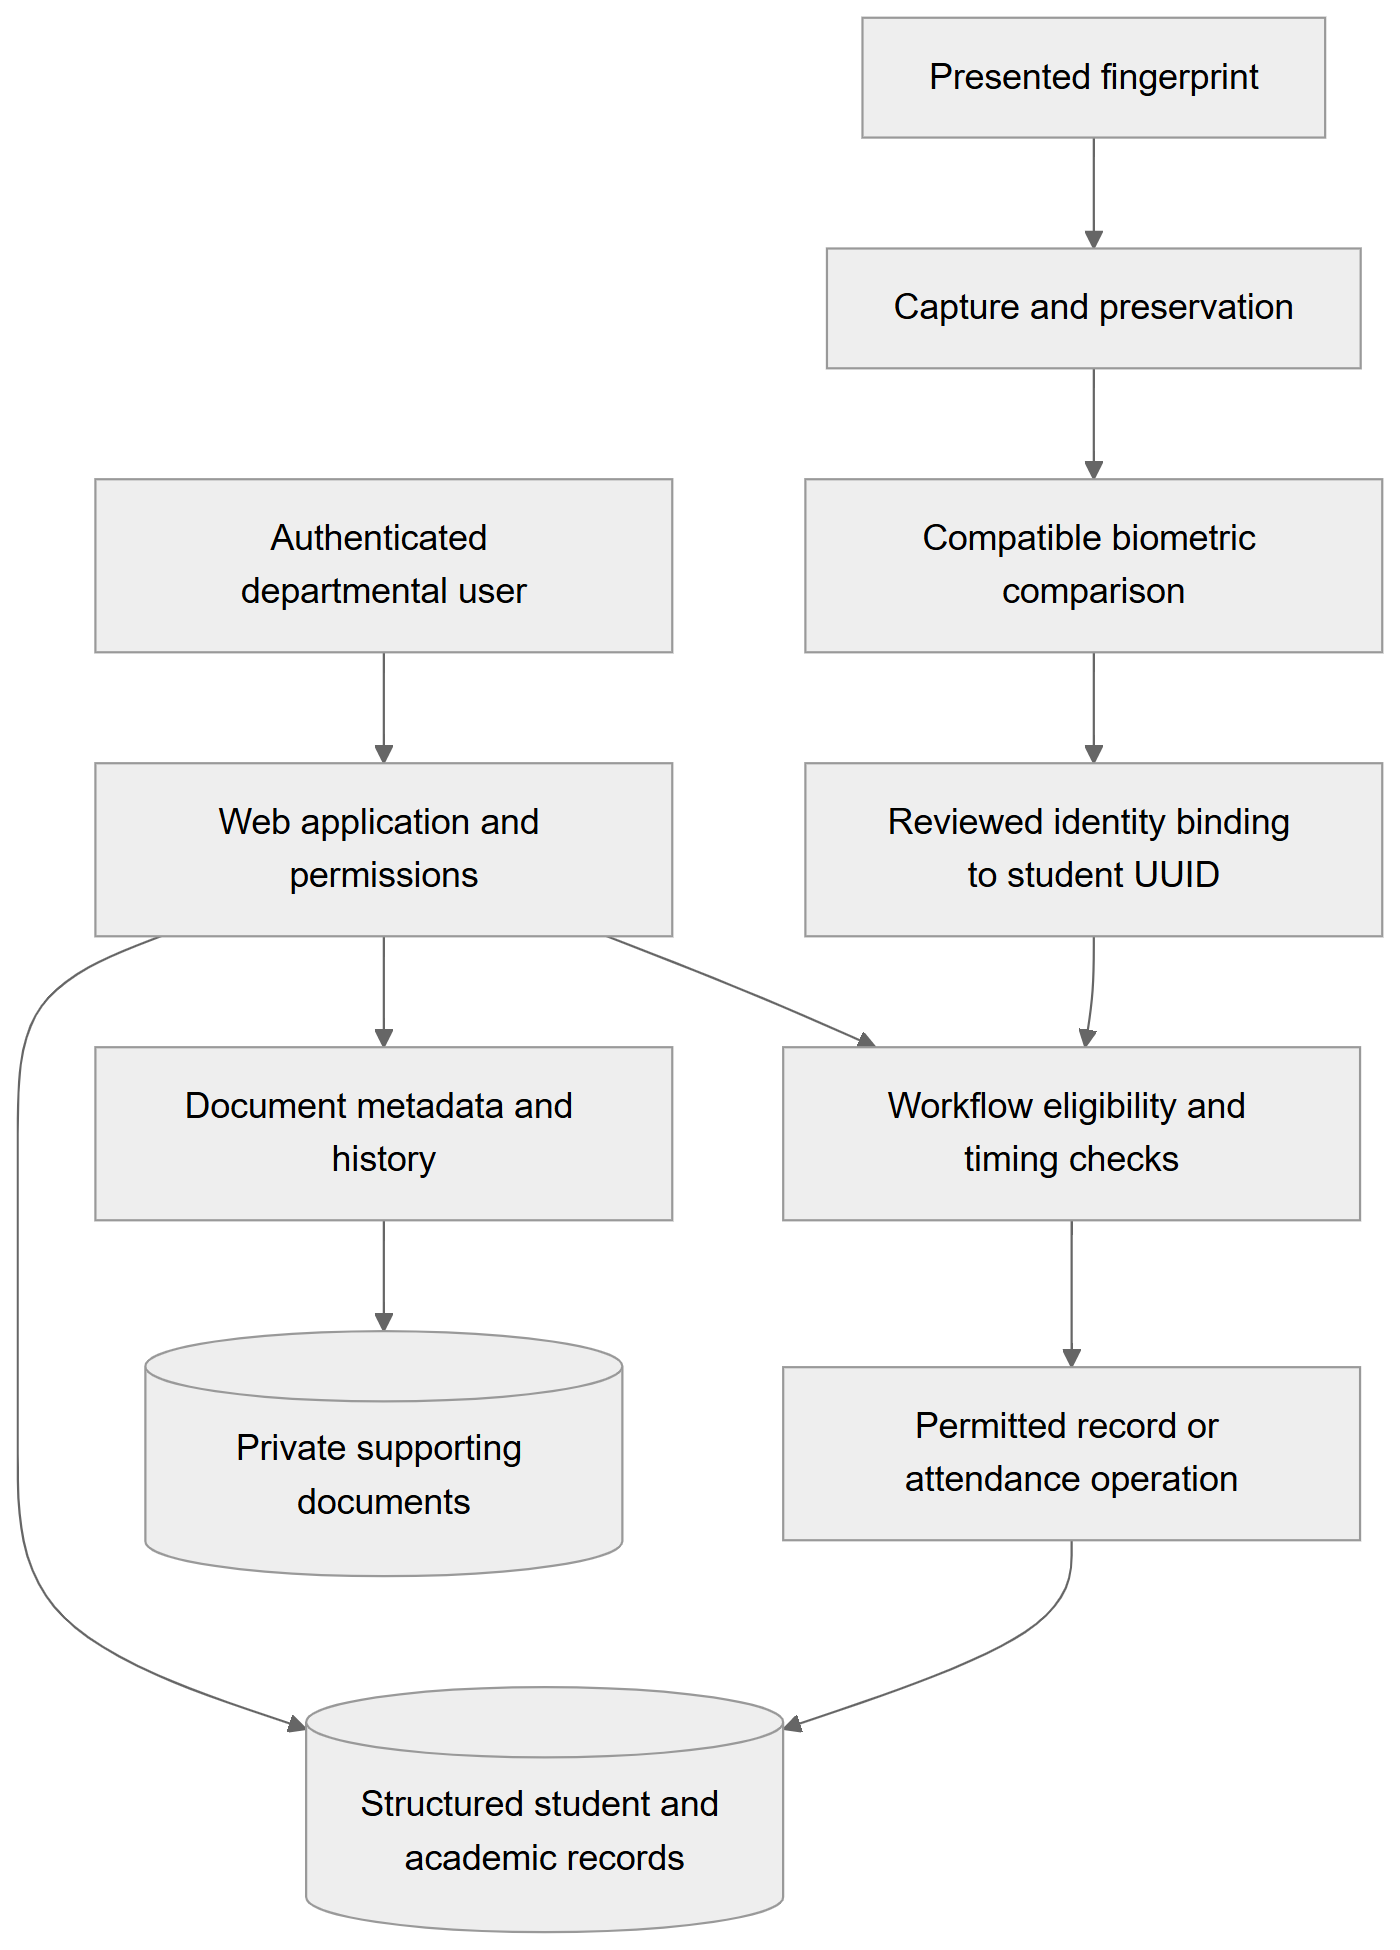
\includegraphics[width=\linewidth,height=0.78\textheight,keepaspectratio]{folder/figure-2_1-conceptual-framework.png}
\caption{Conceptual relationship between filing identity and authorised operations}\label{fig:2-1}
\end{figure}
\clearpage

The student UUID provides the connection between the records and identity domains. Document storage does not depend on using a fingerprint as a filename or primary key. Likewise, a successful comparison does not automatically expose documents or academic results. The application uses the identity outcome within the permissions and requirements of the selected activity.

\section{Research Gap and Project Contribution}~\label{sec:2-10}

The departmental problem reported for this project concerns predominantly hard-copy records that are difficult to retrieve, review, update and correct. The proposed scope includes structured information and uploaded documents. The reviewed literature supplies relevant records-management, academic-information and biometric-integration approaches, but the departmental combination of requirements still needs to be translated into an implemented and evaluated design.

The contribution is therefore framed as the design, implementation and evaluation of an integrated departmental system. Its assessment centres on consistent student identification, controlled records and document operations, appropriate user scope, and the handling of biometric evidence within the selected attendance workflow. The currently developed offline capture and pending-import path also creates a specific integration question: how to preserve unidentified evidence and resolve it later without creating premature attendance, false absences or repeated records.

This is an applied engineering contribution. Any claim that the system is the first to combine fingerprint recognition with a web application, or that it outperforms the reviewed systems, would require evidence beyond the present comparison. The design's value is established by how well it meets the stated departmental requirements and by the limits shown in its evaluation.

\section{Chapter Summary}\label{sec:2-11}

The literature establishes filing and records management as the foundation of the application, with database integrity and access rules governing its operations. Fingerprint recognition supplies identity evidence that must be associated with a stable student record and interpreted within a defined workflow. Previous systems demonstrate relevant approaches but use different architectures and evaluation procedures. Chapter Three translates these principles and departmental requirements into the records model, document design, terminal configuration, integration procedure and evaluation method.

